\documentclass[]{beamer}
\usepackage{amsmath}
\usepackage{tikz}
\usepackage{eurosym}

\title[Pratica 2]{Aula Pratica 2}
\author[P. Fagandini]{Paulo Fagandini}
\institute[ISCAL-IPL]{Lisbon Accounting and Business School}
\date{}

\begin{document}

\maketitle

\frame{
O Miguel tem uma mesada de \euro 120 que pode usar para o consumo mensal de bolos e
maçãs. Assuma que um bolo ($x$) custa \euro 2 e uma maçã ($y$) \euro 1 e que as suas preferências
podem ser descritas pela função utilidade $U=\sqrt{xy}$.
}


\frame{
a) Determine analiticamente a restrição orçamental do Miguel e faça a
representação gráfica do espaço das possibilidades de consumo.

\begin{columns}

    \begin{column}{0.49\textwidth}
        \[2 x+1 y=120\]\[y = \frac{120}{1}-\frac{2}{1}x\]\[y = 120-2x\]
    \end{column}

    \begin{column}{0.49\textwidth}
        \begin{figure}
            \centering

            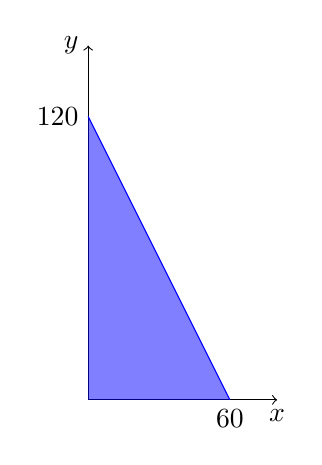
\begin{tikzpicture}[scale = 0.03]

                \onslide<2->{\draw[<->] (0,150) node[left]{$y$} -- (0,0) -- (80,0)node[below]{$x$};}

                \onslide<3->{\draw[blue, domain = 0:60] plot (\x, {120-2*\x});}
                \onslide<4->{
                    \fill[blue, domain=0:60, variable = \x, opacity = 0.5] (0,0) -- plot (\x, {120-2*\x}) -- (0,0) -- cycle;

                    \draw(0, 120) node[left]{$120$};
                    \draw(60,0) node[below]{$60$};
                }

            \end{tikzpicture}
        \end{figure}
    \end{column}
\end{columns}
}

\frame{
b) Represente no gráfico anterior o efeito de uma diminuição do preço dos bolos
para \euro 1.5 na restrição orçamental. Em quanto aumentou a quantidade máxima
que o Miguel pode comprar de bolos? E de maçãs?

\begin{figure}
    \centering

    \begin{tikzpicture}[scale = 0.03]

        \onslide<2->{\draw[<->] (0,150) node[left]{$y$} -- (0,0) -- (100,0)node[below]{$x$};}

        \onslide<3>{
            \draw[blue, domain = 0:60] plot (\x, {120-2*\x});
            \draw(0, 120) node[left]{$120$};
            \draw(60,0) node[below]{$60$};
            }

        \onslide<4->{
            \draw[blue!20, domain = 0:60] plot (\x, {120-2*\x});
            \draw[blue, domain=0:80, variable = \x] plot (\x, {120-1.5*\x});

            \draw(0, 120) node[left]{$120$};
            \draw(80,0) node[below]{$80$};
        }

    \end{tikzpicture}
\end{figure}


}

\frame{
c) Sabemos que o Miguel pode consumir um cabaz com 20 bolos e outro cabaz
com 30 bolos aos novos preços. Quantas maçãs está o Miguel a consumir em
cada um destes cabazes se ambos esgotarem o rendimento do Miguel? Será que
são indiferentes? Quantas maçãs teriam os cabazes se fossem indiferentes? Neste
caso ambos poderiam esgotar o orçamento?

\vspace{1.5em}

\begin{columns}
    \begin{column}{0.49\textwidth}
        Cabaz 1:

        \[1.5\times 20 + 1 \times y = 120\]

        \[y = 90\]

        \[u(20,90)=\sqrt{20\times 90} \approx 42.43\]
    \end{column}

    \begin{column}{0.49\textwidth}
        Cabaz 1:

        \[1.5\times 30 + 1 \times y = 120\]

        \[y = 75\]

        \[u(30,75)=\sqrt{30\times 75} \approx 47.43\]
    \end{column}
\end{columns}
\[\sqrt{30\times y} = 42.43\ \Rightarrow\ y = \frac{42.43^2}{30}=60  \]
}

\frame{
d) Calcule a taxa marginal de substituição entre os cabazes da alínea c) e interprete
o seu significado.
}

\frame{
e) Derive a taxa marginal de substituição (TMS) a partir da função utilidade
apresentada. Qual o valor da TMS no cabaz $(x, y) = (40,40)$? Será que se trata
do cabaz de escolha óptima? Justifique.
}

\frame{
f) Recorrendo à 2ª Lei de Gossen, determine o cabaz de escolha óptima aos preços
iniciais.
}

\frame{
g) Dê um exemplo de um cabaz indiferente ao óptimo. Será que pode pertencer ao
espaço das possibilidades de consumo? Justifique.
}

\frame{
h) Determine a equação que descreve a curva de indiferença que contém o cabaz de
escolha óptima.
}

\frame{
i) Se o preço dos bolos aumentar para \euro 2.5, o que espera que aconteça à
quantidade consumida deste bem?
}

\end{document}
